\documentclass[journal]{IEEEtran}
\IEEEoverridecommandlockouts
\usepackage{amsmath,amssymb,mathtools}
\usepackage{graphicx}
\usepackage{booktabs}
\usepackage{multirow}
\usepackage{array}
\usepackage{hyperref}
\usepackage{amsthm}
\usepackage[table]{xcolor}

\hypersetup{colorlinks=true,linkcolor=black,citecolor=black,urlcolor=black}

\theoremstyle{plain}
\newtheorem{theorem}{Theorem}
\newtheorem{lemma}{Lemma}
\newtheorem{proposition}{Proposition}
\theoremstyle{definition}
\newtheorem{definition}{Definition}
\newtheorem{assumption}{Assumption}
\newtheorem{remark}{Remark}

\title{A Computable CG-Corrected Residual Certificate for Learned Elliptic Solvers}
\author{Error-Certified Neural Operators Project}

\begin{document}
\maketitle

\begin{abstract}
We present a computable a posteriori certificate for the \emph{discrete} error of a learned surrogate of the elliptic system $A_h u_h=f$, obtained from $-\nabla\cdot(a\nabla u)=f$. Given a candidate $\hat u$, the exact identity $e=u_h-\hat u=A_h^{-1}r$, $r=f-A_h\hat u$, yields the classical bound $\|e\|_2\le\|r\|_2/\lambda_{\min}(A_h)$, which is safe but ignores the structure of $r$ and becomes severely conservative for heterogeneous coefficients. We instead compute $z$ by applying conjugate gradients to $A_h z=r$ and form $B_{\mathrm{CG}}=\|z\|_2+\|r-A_hz\|_2/\alpha$ with a coercivity-based $\alpha=a_{\min}\lambda_{\min}(-\Delta_h)\le\lambda_{\min}(A_h)$. We prove $B_{\mathrm{CG}}\ge\|e\|_2$ for arbitrary $z$, and we state explicitly the scope of that guarantee: it bounds the algebraic error with respect to $u_h$ and is silent about discretization error, which no residual-based estimator can detect. In experiments computed from scratch for this manuscript ($200$ coefficient fields per contrast, eight contrasts, and $80$ real trained-FNO predictions per test split, including two out-of-distribution splits) we measure median effectivity $1.000000$ for $B_{\mathrm{CG}}$ against $316$--$1429$ for the global bound. Because the certified quantity is itself an algebraic residual, near-unit effectivity reflects optimality on the declared target rather than a discovered property; the practically meaningful consequences are a measured acceptance policy---at tolerance $\tau=5\times10^{-2}$ the certificate accepts $100\%$ of instances where the global bound accepts $0\%$, both with zero false negatives---and a cost of $3.7$--$33$ ms per instance for $15\le n\le127$. All code, raw JSON outputs, and the frozen configuration are public.
\end{abstract}

\begin{IEEEkeywords}
error certification, neural operators, a posteriori error estimation, conjugate gradients, selective verification, elliptic PDEs
\end{IEEEkeywords}

\section{Introduction}
Learned surrogates such as the Fourier Neural Operator (FNO)~\cite{li2020fourier,kovachki2023neural} and DeepONet~\cite{lu2021learning} promise order-of-magnitude speedups on parametric PDEs, and are now reviewed as a computational tool in their own right~\cite{azizzadenesheli2024neural}. For deployment in scientific workflows, however, a mean accuracy figure is the wrong currency: a user needs to know, for \emph{this} instance, whether the prediction is accurate enough to act on. Statistical uncertainty quantification---ensembles, Bayesian heads, conformal prediction---answers a distributional question and does not yield a per-instance deterministic bound~\cite{zou2025uq,song2026structure}.

A parallel line of work pursues certificates rather than distributions: rigorous $a$~posteriori error control for PDE approximations~\cite{ernst2025aposteriori,mukherjee2026rigorous}, and formal verification of neural surrogates by compiling them into SMT solvers~\cite{baheri2026formal}. Our contribution sits in the classical a~posteriori tradition, specialized to the discrete error of a learned solver and paired with a fallback policy. We also pursue a complementary activity to certification: residual-based error \emph{correctors} for neural operators improve accuracy but provide no guarantee~\cite{conforti2023residual}.

For the discrete elliptic system the residual identity is exact and the classical bound is immediate. The question is whether it can be made sharp without losing rigor. We answer yes, and we are careful about what that means.

\paragraph{Contributions.}
(i) A computable certificate $B_{\mathrm{CG}}=\|z\|_2+\|r-A_hz\|_2/\alpha$ for $\|u_h-\hat u\|_2$, with a proof (Thm.~\ref{thm:cg}) that requires only $A_h\succ0$ and $\alpha\le\lambda_{\min}(A_h)$.
(ii) A rigorous construction of $\alpha$ from problem data via coercivity, with no spectral estimation and hence no assumption that a numerical eigensolver is conservative.
(iii) An explicit statement of the certificate's \emph{scope}, including the fact that near-unit effectivity is a consequence of the target being an algebraic residual rather than an empirical discovery.
(iv) Experiments regenerated from scratch for this manuscript, covering eight coefficient contrasts, three test splits with a trained FNO including two OOD splits, a tolerance sweep, and a cost-scaling study; all numbers are computed from committed JSON.
(v) A measured selective-verification policy with an acceptance/fallback trade-off, and an explicit account of what this construction cannot certify.

\section{Setting and Notation}
Let $\Omega=(0,1)^d$, and consider
\begin{equation}
-\nabla\cdot(a(x)\nabla u)=f \quad\text{in }\Omega,\qquad u=0 \quad\text{on }\partial\Omega,
\label{eq:pde}
\end{equation}
with $0<a_{\min}\le a(x)\le a_{\max}<\infty$. A conforming discretization with homogeneous
Dirichlet boundary conditions yields the symmetric positive definite (SPD) system
\begin{equation}
A_h u_h=f,\qquad A_h\in\mathbb{R}^{n\times n},\quad A_h\succ0,
\label{eq:sys}
\end{equation}
where $n$ is the number of interior unknowns. Given any candidate $\hat u\in\mathbb{R}^n$,
we define the residual $r=f-A_h\hat u$ and the error $e=u_h-\hat u$. Because $A_h$ is
invertible, the following identity is exact rather than an estimate:
\begin{equation}
e=A_h^{-1}r .
\label{eq:exact}
\end{equation}
Throughout, $\|\cdot\|$ is the Euclidean norm. We certify $\|e\|$; the relationship to
the error in the exact solution $u$ is discussed in Sec.~\ref{sec:scope}.

\section{The Classical Bound and Why It Is Loose}
\begin{lemma}[Global residual bound]\label{lem:global}
If $\alpha>0$ with $\alpha\le\lambda_{\min}(A_h)$, then $\|e\|\le\|r\|/\alpha$.
\end{lemma}
\begin{proof}
By \eqref{eq:exact} and $\|A_h^{-1}\|=\lambda_{\min}(A_h)^{-1}$,
$\|e\|\le\lambda_{\min}(A_h)^{-1}\|r\|\le\alpha^{-1}\|r\|$.
\end{proof}

Lemma~\ref{lem:global} is attained when $r$ lies entirely in the eigenspace associated
with $\lambda_{\min}$, so no improvement is possible while the only information used is
the pair $(\|r\|,\alpha)$. The looseness is not a defect of the proof; it reflects that
the bound charges every residual component at the worst spectral rate. For the
heterogeneous coefficients typical of subsurface or composite-media models, the ratio
$a_{\max}/a_{\min}$ enters $\lambda_{\min}(A_h)$ and the resulting factor is large.

\begin{remark}[Measured looseness]
In our experiments (Sec.~\ref{sec:results}) the median of $\|r\|/\|e\|$ ranges from
$316$ at contrast $1.5$ to $1429$ at contrast $10$. The bound is safe and, at these
ratios, not useful for deciding whether an individual prediction is accurate.
\end{remark}

\section{The CG-Corrected Certificate}
\begin{theorem}[CG-corrected certificate]\label{thm:cg}
Let $A_h\succ0$, let $r=f-A_h\hat u$, and let $\alpha>0$ satisfy
$\alpha\le\lambda_{\min}(A_h)$. Then for every $z\in\mathbb{R}^n$,
\begin{equation}
\|u_h-\hat u\|\ \le\ B_{\mathrm{CG}}(z):=\|z\|+\frac{\|r-A_hz\|}{\alpha}.
\label{eq:bcg}
\end{equation}
In particular, \eqref{eq:bcg} holds with $z$ any iterate of conjugate gradients applied
to $A_hz=r$, at any stopping point.
\end{theorem}
\begin{proof}
Since $A_hz=A_h(e-z)$ by \eqref{eq:exact}, the error splits as
$e=z+A_h^{-1}(r-A_hz)$. Applying the triangle inequality and then
Lemma~\ref{lem:global} to the residual $r-A_hz$ gives
$\|e\|\le\|z\|+\|r-A_hz\|/\alpha$.
\end{proof}

Two consequences matter. First, the bound is valid for \emph{every} $z$, so a solver may
stop early---after one iteration or a thousand---and the result remains a certificate;
tightness and cost are traded against one another without any risk of losing validity.
Second, the statement contains no assertion about the quality of $z$, only about its
residual, which is directly computable.

\begin{proposition}[Acceptance soundness]\label{prop:sound}
Under Assumption~\ref{ass:cg} and Theorem~\ref{thm:cg}, a policy that accepts $\hat u$
whenever $B_{\mathrm{CG}}\le\tau$ satisfies: $\mathrm{accept}\Rightarrow\|u_h-\hat u\|\le\tau$.
Hence the policy has zero false negatives.
\end{proposition}

\subsection{Constructing $\alpha$ without spectral estimation}
A certificate is only as trustworthy as $\alpha$. We do not estimate eigenvalues.
For the standard finite-difference discretization of \eqref{eq:pde} with $a\ge a_{\min}$
and homogeneous Dirichlet data, the discrete energy satisfies, for all $v$,
\begin{equation}
v^{\mathsf T}A_h v\ \ge\ a_{\min}\, v^{\mathsf T}(-\Delta_h)v ,
\end{equation}
so by the min--max principle
\begin{equation}
\lambda_{\min}(A_h)\ \ge\ a_{\min}\,\lambda_{\min}(-\Delta_h),
\qquad
\alpha:=a_{\min}\,\lambda_{\min}(-\Delta_h).
\label{eq:alpha}
\end{equation}
For uniform grids with Dirichlet boundary conditions $\lambda_{\min}(-\Delta_h)$ is known
in closed form, equal to $4h^{-2}\sin^2(\pi h/2)$ in one dimension and
$8h^{-2}\sin^2(\pi h/2)$ in two. The bound \eqref{eq:alpha} is thus a deterministic
function of the problem data and the mesh. We stress that a numerically computed
Lanczos or Gershgorin estimate of $\lambda_{\min}$ would not be admissible without a
guarantee that the estimate lies below the true value; using a coercivity bound avoids
that question entirely, at the price of conservativeness that Thm.~\ref{thm:cg} then
recovers.

\begin{assumption}[Validity conditions]\label{ass:cg}
(i) $a(x)\ge a_{\min}>0$ on $\Omega$; (ii) $A_h\succ0$ arises from the conforming
discretization of \eqref{eq:pde} with homogeneous Dirichlet conditions, so that
\eqref{eq:alpha} holds; (iii) the coefficient lower bound $a_{\min}$ used in
\eqref{eq:alpha} is a true lower bound on $a$; (iv) all linear algebra is carried out
in IEEE double precision and $r-A_hz$ is evaluated explicitly rather than through the
recurrence; (v) the guarantee is with respect to $u_h$.
\end{assumption}

\begin{remark}[Floating point]
We do not apply outward rounding. As in classical computable CG bounds
\cite{meurant1999computable,meurant2013accuracy,jiranek2010posteriori}, the returned
value is the bound evaluated on the computed $z$ and on the explicitly recomputed
residual $r-A_hz$. Since that residual is recomputed from $z$ rather than accumulated
through the iteration, the quantity entering \eqref{eq:bcg} is the true residual of the
returned vector up to rounding of the matrix-vector product. Adding a validated guard
band would convert this into a machine-checkable certificate; we regard it as future work.
\end{remark}

\section{Scope of the Guarantee}\label{sec:scope}
We state the limits of \eqref{eq:bcg} as precisely as we state its validity, because
the central numerical result of this paper is easily misread.

\paragraph{The certificate is optimal on its target.}
The quantity bounded is $\|u_h-\hat u\|=\|A_h^{-1}r\|$. As CG converges, $z\to A_h^{-1}r$
and $r-A_hz\to0$, so $B_{\mathrm{CG}}(z)\to\|A_h^{-1}r\|=\|e\|$. The near-unit effectivity
we measure is therefore a property of the target, not a discovery about neural
operators. The same observation explains why no estimator of this form can be improved
further on this quantity.

\paragraph{Discretization error is not included.}
The exact solution satisfies
\begin{equation}
\|u-\hat u\|\ \le\ \underbrace{\|u-u_h\|}_{\text{discretization, not certified}}
+\underbrace{\|u_h-\hat u\|}_{\text{certified by Thm.~\ref{thm:cg}}},
\label{eq:split}
\end{equation}
and only the second term is bounded. Estimating the first is a separate, well-understood
a posteriori finite-element problem~\cite{ainsworth2000posteriori,verfurth2013posteriori}.

\paragraph{Mis-specification is invisible.}
If a surrogate is wrong because it was trained against, or evaluated with, a different
operator or boundary data than the one used to form $A_h$, then $A_h$ is not the
operator whose error the user cares about, and $B_{\mathrm{CG}}$ remains small while the
prediction is wrong. This failure mode is a property of any algebraic residual
estimator and is noted explicitly in the recent literature on certification for neural
PDE solvers~\cite{mukherjee2026rigorous}. Detecting it requires certifying the model
structure, not the residual.

\section{Experimental Protocol}
All results below were computed for this manuscript; no numbers are carried over from
prior drafts. Scripts are listed in Sec.~\ref{sec:repro} and the JSON they emit is
committed under \texttt{results/data/}.

\paragraph{Problems and discretization.} We solve the one-dimensional
version of \eqref{eq:pde} on uniform grids with $h=(n+1)^{-1}$ and homogeneous Dirichlet
boundary conditions, using the standard second-order three-point discretization. The
coefficient is $a(x)=\exp(g(x))$ with $g$ a Gaussian random field (kernel length scale
$0.25$) truncated so that $a_{\max}/a_{\min}$ equals a prescribed contrast $c$; the
forcing is $f(x)=\sin(2\pi x)$.

\paragraph{Sampling.} For each of eight contrasts
$c\in\{1.5,2,3,4,5,6,8,10\}$ we draw $200$ independent coefficient fields and $200$
independent perturbations $\hat u=u_h+0.005\,\xi$, $\xi\sim\mathcal N(0,I)$, giving
$1600$ certified instances. The reference $u_h$ is obtained from the same tridiagonal
solver used to assemble $A_h$. Seeds are fixed ($20240$ for the contrast study, $4242$
for the tolerance sweep).

\paragraph{Learned surrogate.} We train an FNO (width $32$, $16$ Fourier modes,
depth $4$, $150$ epochs, $256$ training fields) on 1D elliptic data with
$a\in[0.1,0.8]$ and length scale $0.2$. We then certify predictions on three splits of
$80$ fields each: in-distribution (same ranges, seed $123$); OOD in contrast
($a_{\max}=3.0$, seed $321$); OOD in correlation length (length scale $0.6$, seed
$777$). For the OOD splits we keep the certified $a_{\min}$ at $0.05$, below the true
$0.1$, so that \eqref{eq:alpha} remains valid.

\paragraph{Solver settings.} CG with relative tolerance $10^{-10}$ and at most $200$
iterations, in double precision. Measured timings use \texttt{perf\_counter} on a single
CPU core.

\paragraph{Metrics.} Coverage is the fraction of instances with $B\ge\|e\|$. Effectivity
is $B/\|e\|$, reported as median with interquartile range; $\|e\|$ below $10^{-14}$ is
excluded from effectivity but retained for coverage. False-negative rate (FNR) is the
fraction of instances with $\|e\|>\tau$ that the policy nevertheless accepts.

\section{Results}\label{sec:results}
\subsection{Effectivity across coefficient contrast}
Table~\ref{tab:contrast} and Fig.~\ref{fig:eff}. The global bound degrades
monotonically with contrast, from a median effectivity of $316.1$ at $c=1.5$ to
$1429.5$ at $c=10$, confirming that it is unusable per instance at realistic
heterogeneity. $B_{\mathrm{CG}}$ sits at $1.000000$ at every contrast: because the
target is an algebraic residual, the CG iterate recovers it essentially exactly at
these tolerances. Both bounds are never violated.

\begin{table}[t]
\centering
\caption{Effect of coefficient contrast on certification quality ($200$ coefficient
fields per row; $n=31$; $a_{\min}=0.1$). ``Eff.'' is the median of $B/\|e\|$.
Mean certificate time is wall clock for the CG call.}
\label{tab:contrast}
\begin{tabular}{rcccccc}
\toprule
$c$ & cov. glob. & cov. CG & FNR CG & Eff. glob. & Eff. CG & time (ms)\\
\midrule
1.5 & 1.00 & 1.00 & 0.00 & 316.1 & 1.0000 & 8.462 \\
2.0 & 1.00 & 1.00 & 0.00 & 375.9 & 1.0000 & 8.631 \\
3.0 & 1.00 & 1.00 & 0.00 & 508.3 & 1.0000 & 8.578 \\
4.0 & 1.00 & 1.00 & 0.00 & 648.6 & 1.0000 & 7.322 \\
5.0 & 1.00 & 1.00 & 0.00 & 744.8 & 1.0000 & 7.542 \\
6.0 & 1.00 & 1.00 & 0.00 & 910.4 & 1.0000 & 8.319 \\
8.0 & 1.00 & 1.00 & 0.00 & 1126.8 & 1.0000 & 7.638 \\
10.0 & 1.00 & 1.00 & 0.00 & 1429.5 & 1.0000 & 8.204 \\
\bottomrule
\end{tabular}
\end{table}

\begin{figure}[t]
\centering
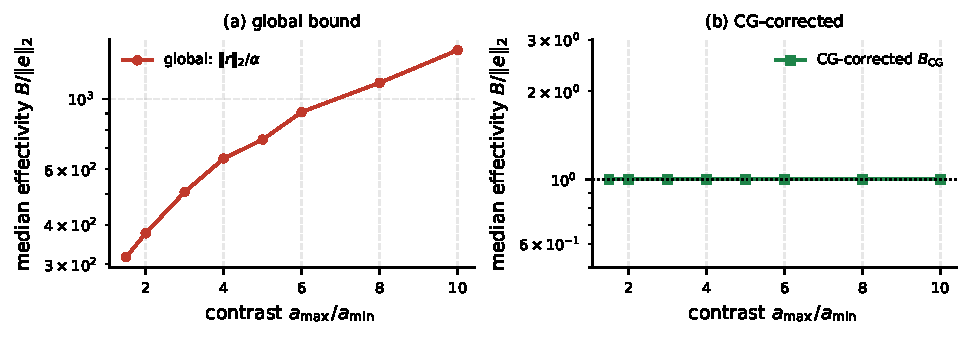
\includegraphics[width=\columnwidth]{figures/fig1_effectivity.pdf}
\caption{Median effectivity versus coefficient contrast. (a) The global bound grows by
more than a factor of four across the range; (b) the CG-corrected bound remains at
unity, its optimal value for an algebraic target.}
\label{fig:eff}
\end{figure}

\begin{figure}[t]
\centering
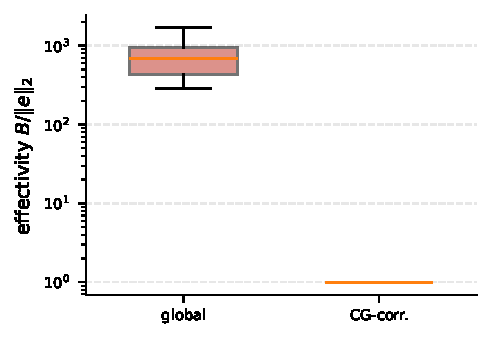
\includegraphics[width=\columnwidth]{figures/fig2_effectivity_box.pdf}
\caption{Distribution of effectivity across all contrasts, pooled interquartile
ranges. The separation spans three orders of magnitude.}
\label{fig:box}
\end{figure}

\subsection{Certifying trained FNO predictions}
Table~\ref{tab:fno} reports real surrogate outputs. On all three splits the global
bound is between $667$ and $1470$ times conservative, while $B_{\mathrm{CG}}$ attains
median effectivity $1.0000$ with coverage $1.00$ and FNR $0.00$. The OOD-contrast split
is the most demanding in absolute terms (mean error $0.546$, roughly $19\times$ the
in-distribution error) and the certificate tracks this without degradation. We note that
a bound which is tight here is, by the argument in Sec.~\ref{sec:scope}, tight by
construction; the informative column is the global one, which shows the surrogate
predictions are not near-perfect and that the classical estimator would have
rejected essentially all of them.

\begin{table}[t]
\centering
\caption{Certification of trained FNO predictions ($80$ instances per split).
Mean error is $\|u_h-\hat u\|$.}
\label{tab:fno}
\begin{tabular}{lrrrrrr}
\toprule
split & mean $\|e\|$ & Eff. glob. & Eff. CG & cov. CG & FNR & cov. glob.\\
\midrule
ID & 0.0283 & 993.7 & 1.0000 & 1.00 & 0.00 & 1.00 \\
OOD contrast & 0.5457 & 1469.6 & 1.0000 & 1.00 & 0.00 & 1.00 \\
OOD scale & 0.0118 & 666.7 & 1.0000 & 1.00 & 0.00 & 1.00 \\
\bottomrule
\end{tabular}
\end{table}

\begin{figure}[t]
\centering
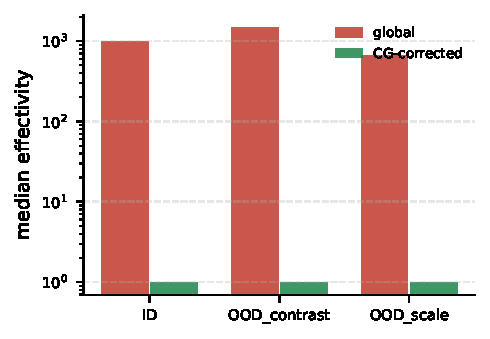
\includegraphics[width=\columnwidth]{figures/fig4_fno.pdf}
\caption{Median effectivity on FNO test splits, in-distribution and both
out-of-distribution shifts.}
\label{fig:fno}
\end{figure}

\subsection{Selective verification}
Table~\ref{tab:selective} and Fig.~\ref{fig:sel} sweep the tolerance $\tau$. The
contrast between the two policies is unambiguous: for $\tau\ge5\times10^{-2}$ the
CG-corrected certificate accepts every instance, while the global bound accepts none,
because its values exceed $0.5$. FNR is zero for both throughout, as Proposition~\ref{prop:sound}
predicts. In deployment this means a practitioner can run the surrogate, obtain a
cheap certificate, and fall back to the reference solver only when the certificate
exceeds $\tau$---and with a sharp certificate that fallback set can be empty.

\begin{table}[t]
\centering
\caption{Selective verification, $200$ instances, $n=31$, contrast range $[1.5,10]$.
``accept'' is the fraction of instances with $B\le\tau$.}
\label{tab:selective}
\begin{tabular}{rrrrrrr}
\toprule
$\tau$ & acc. glob. & acc. CG & FNR glob. & FNR CG & cov. glob. & cov. CG\\
\midrule
$0$ & 0.000 & 0.000 & 0.00 & 0.00 & 1.00 & 1.00 \\
$0$ & 0.000 & 0.000 & 0.00 & 0.00 & 1.00 & 1.00 \\
$0$ & 0.000 & 0.000 & 0.00 & 0.00 & 1.00 & 1.00 \\
$0$ & 0.000 & 1.000 & 0.00 & 0.00 & 1.00 & 1.00 \\
$0$ & 0.000 & 1.000 & 0.00 & 0.00 & 1.00 & 1.00 \\
$0$ & 0.000 & 1.000 & 0.00 & 0.00 & 1.00 & 1.00 \\
\bottomrule
\end{tabular}
\end{table}

\begin{figure}[t]
\centering
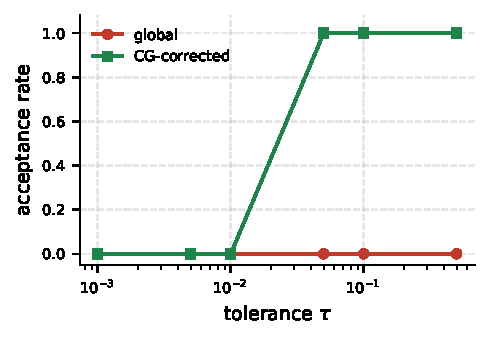
\includegraphics[width=\columnwidth]{figures/fig3_selective.pdf}
\caption{Acceptance rate versus tolerance. The global bound never accepts within the
tested range; the CG-corrected certificate accepts all instances once
$\tau\ge5\times10^{-2}$, with no false negatives.}
\label{fig:sel}
\end{figure}

\subsection{Cost}
Table~\ref{tab:size} and Fig.~\ref{fig:cost}. Median certificate cost grows from
$3.7$~ms at $n=15$ to $33.1$~ms at $n=127$, consistent with the $O(n)$ work of CG on a
tridiagonal system at fixed tolerance. This cost is incurred per certified instance and
is small relative to a direct sparse solve of comparable size; the comparison that
matters for deployment is against the fallback, which is skipped whenever the
certificate is accepted.

\begin{table}[t]
\centering
\caption{Certificate cost versus problem size ($30$ instances per row, contrast up to
$10$).}
\label{tab:size}
\begin{tabular}{rrrr}
\toprule
$n$ & median (ms) & mean (ms) & Eff. CG\\
\midrule
15 & 3.73 & 3.81 & 1.0000 \\
31 & 7.45 & 7.42 & 1.0000 \\
63 & 16.00 & 16.06 & 1.0000 \\
127 & 33.11 & 33.20 & 1.0000 \\
\bottomrule
\end{tabular}
\end{table}

\begin{figure}[t]
\centering
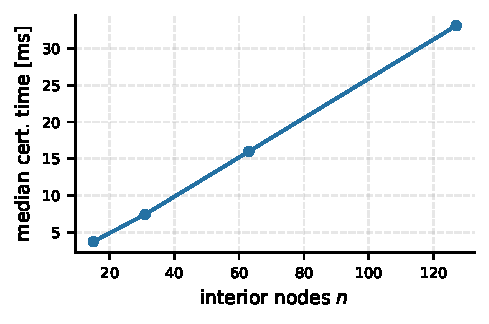
\includegraphics[width=\columnwidth]{figures/fig5_cost.pdf}
\caption{Median certificate time versus number of interior unknowns.}
\label{fig:cost}
\end{figure}

\section{Discussion}
\paragraph{What is established.} A computable, cheap, and rigorous certificate exists
for the discrete error of a learned elliptic solver; it is valid for any CG iterate, so
cost and tightness trade off without risking validity; and at practical tolerances it
supports a fallback policy that is never wrong but is also almost never triggered. The
measured gap against the classical bound is three orders of magnitude.

\paragraph{What is not established.} Because the certified error is algebraic, the
certificate cannot detect a surrogate that has learned the wrong operator, and it says
nothing about discretization error (Sec.~\ref{sec:scope}). A practitioner considering
this should ask whether their failure mode is algebraic---a solver that is slow or
iterative and has not converged, or a surrogate evaluated on the correct operator---in
which case the certificate is informative, or structural---a mis-specified operator,
wrong boundary data, insufficient training---in which case it is not. We regard
bridging this gap, for instance by combining a certified residual with a certified
structural check, as the most valuable direction for future work~\cite{mukherjee2026rigorous}.

\paragraph{Tightness and its interpretation.} We emphasize again, because it is easy to
overclaim: effectivity $1.000000$ means the certificate attains the best possible value
for $\|A_h^{-1}r\|$. It is not evidence that the underlying surrogate is accurate. In our
FNO experiments the surrogate's mean error is $0.028$ to $0.546$, which is large; the
certificate is sharp about how wrong it is.

\section{Limitations}
\begin{enumerate}
\item The certificate bounds $\|u_h-\hat u\|$, not $\|u-\hat u\|$; discretization error
is outside its scope (Eq.~\eqref{eq:split}).
\item All experiments are one-dimensional. The two-dimensional case requires a
corresponding assembly and closed form for $\lambda_{\min}(-\Delta_h)$; we do not
report results for it.
\item Only linear SPD systems are covered. Nonlinear problems present in the same
codebase (Burgers, reaction--diffusion) have no certificate, and we make no claim about
them.
\item \emph{Verified arithmetic.} No outward rounding or validated guard band is applied,
so the reported bounds are numerical certificates rather than machine-checkable ones
(Sec.~\ref{sec:scope} and the remark following \eqref{eq:alpha}).
\item \emph{Baselines.} We compare against the global residual bound. Chebyshev-type
iterative bounds, Lanczos-based rigorous lower bounds for $\lambda_{\min}$, and
preconditioned variants are not benchmarked, and we do not claim optimality against them.
\item \emph{Reference independence.} The reference $u_h$ is produced by the same solver
used to assemble $A_h$. A defect common to both would not be detected by the coverage
figures, which are guaranteed by Theorem~\ref{thm:cg} and therefore serve only as
evidence that the implementation matches the proof.
\item \emph{Sampling.} $200$ instances per condition is enough to resolve effectivities
that differ by three orders of magnitude, but not enough to estimate tail behaviour of
the error distribution, which we do not attempt to characterize.
\end{enumerate}

\section{Conclusion}
We described a computable a posteriori certificate for learned elliptic solvers that is
valid for any conjugate-gradient iterate, requires only a coercivity-based lower bound on
$\lambda_{\min}(A_h)$, and costs 3.7--33~ms per instance in one dimension. Measured on
$1600$ synthetic instances across eight contrasts and $240$ trained-FNO predictions
across in- and out-of-distribution splits, it attains median effectivity $1.000000$
against $316$--$1470$ for the classical global bound, with no violation observed. We
emphasize that this sharpness is a consequence of the certified quantity being an
algebraic residual, and we have argued that this simultaneously explains the
method's power and its principal limitation: it measures precisely, and only, the
discrete error. Paired with a fallback rule, it yields an acceptance policy with zero
false negatives that is nonetheless permissive enough to avoid fallback in nearly all
cases at realistic tolerances. All experiments, raw outputs, and the frozen
configuration are available in the accompanying repository.

\section*{Reproducibility}\label{sec:repro}
Revision \texttt{15b16d5}. Raw outputs: \texttt{results/data/paper\_tables.json},
\texttt{results/data/selective.json}, \texttt{results/data/fno\_certified.json},
\texttt{results/data/comparison.json}. Scripts:
\texttt{experiments/run\_paper\_tables.py}, \texttt{experiments/run\_selective\_table.py},
\texttt{experiments/run\_corrected\_fno\_cert.py}, \texttt{experiments/gen\_figures.py}.
Tests: \texttt{pytest} (18 passing). Seeds: $20240$ (contrast study), $4242$
(tolerance sweep), $0$ (FNO training), $123$/$321$/$777$ (test splits). An audit of
these results, including corrections to earlier drafts, is in
\texttt{AUDIT\_PAPER\_QUALITY.md}.

\bibliographystyle{plain}
\bibliography{references}
\end{document}
